\documentclass[14pt]{extarticle}
\usepackage[english,ukrainian]{babel}
\usepackage[utf8]{inputenc}
\usepackage[T1]{fontenc}

\usepackage{amsmath,amssymb}
\usepackage{parskip}
\usepackage{graphicx}
\usepackage{xcolor}
\usepackage{tcolorbox}
\tcbuselibrary{skins}
\usepackage[framemethod=tikz]{mdframed}
\usepackage{chngcntr}
\usepackage{enumitem}
\usepackage{hyperref}
\usepackage{float}
\usepackage{subfig}
\usepackage{esint}
\usepackage[top=2.5cm, left=3cm, right=3cm, bottom=4.0cm]{geometry}
\usepackage[table]{xcolor}
\usepackage{algorithm}
\usepackage{algpseudocode}
\usepackage{listings}

\title{Домашня робота з курсу ``Теоретична механіка''}
\author{Студента 3 курсу групи МП-31 Захарова Дмитра}
\date{\today}

\begin{document}

\maketitle
\section*{Завдання 12.32}

\textbf{Умова.} Див. рис. \ref{fig:1}.
\begin{figure}[H]
    \centering
    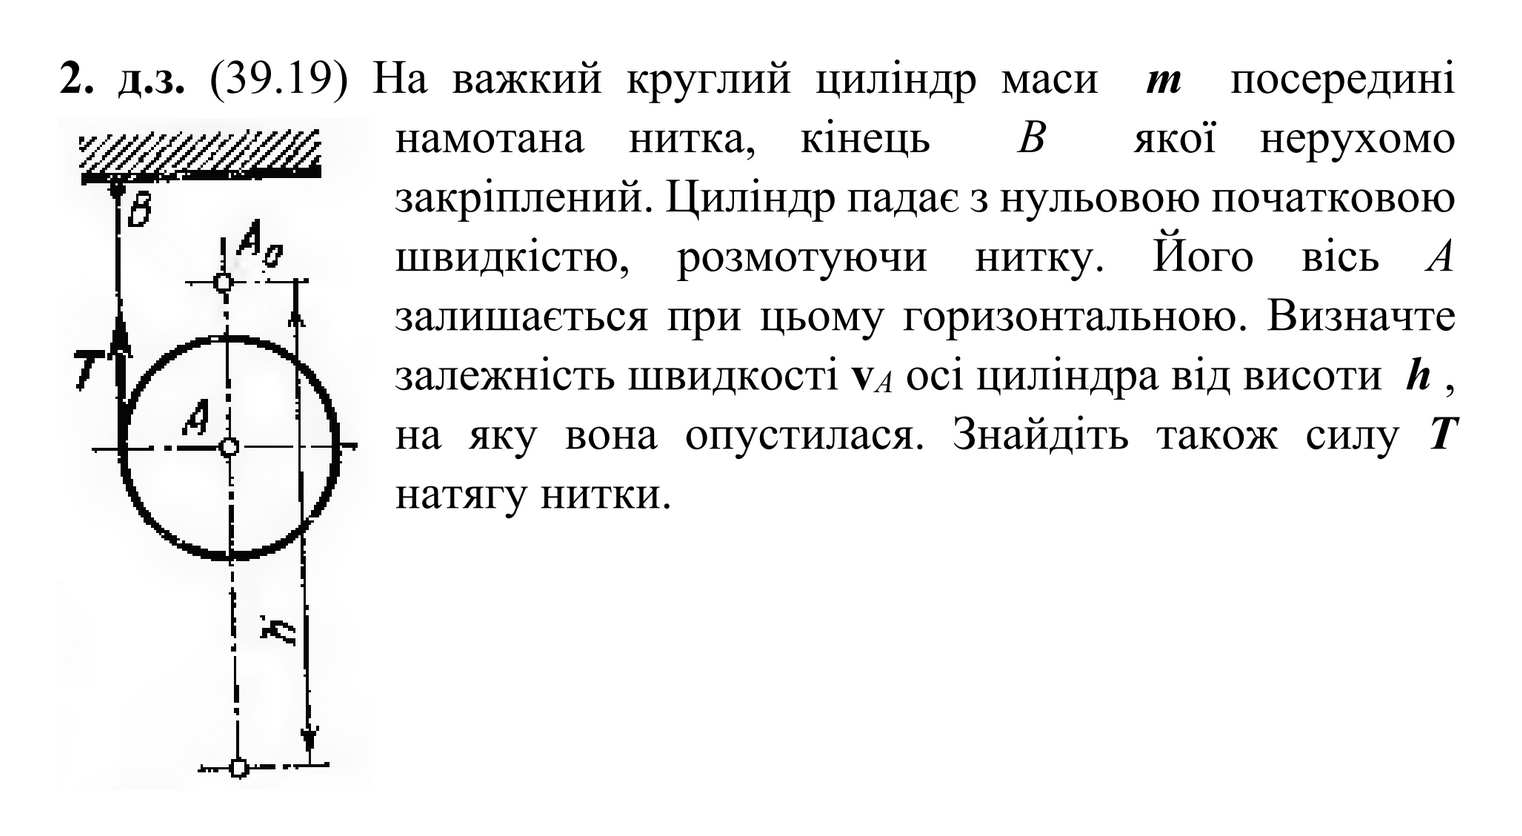
\includegraphics[width=\textwidth]{images/hw_12/problem.png}
    \caption{Умова до завдання}
    \label{fig:1}
\end{figure}
\pagebreak
\textbf{Розв'язок.} Нехай в деякий момент вісь циліндра має швикість $v$. В такому разі кутова швидкість $\omega=\frac{v}{R}$. Отже повна кінетична енергія:
\[
W_k = \frac{mv^2}{2} + \frac{I\omega^2}{2} = \frac{mv^2}{2} + \frac{mR^2}{4} \cdot \left(\frac{v}{R}\right)^2 = \frac{3mv^2}{4}
\]
Розглянемо дуже малий проміжок часу. Тожі, зміна кінетичної енергії набувається за рахунок зміни потенціальної енергії за малий проміжок часу:
\[
\frac{3mv \Delta v}{2} = mg \Delta h \implies \frac{3}{2} \cdot \frac{\Delta v}{\Delta t} = g \implies a = \frac{2g}{3}
\]
З іншого боку, за другим законом Ньютона:
\[
ma = mg - T \implies T = \frac{mg}{3}
\]
Знайдемо швидкість як функцію від висоти. Швидкість через час $t$ дорівнює $v(t)=at = \frac{2gt}{3}$. З іншого боку, функція висоти від часу $h = \frac{at^2}{2}=\frac{gt^2}{3} \implies t = \sqrt{\frac{3h}{g}}$. Тому
\[
v(h) = \frac{2g}{3}\sqrt{\frac{3h}{g}} = 2\sqrt{\frac{gh}{3}}
\]

\textbf{Відповідь.} $v = 2\sqrt{\frac{gh}{3}},\;T=\frac{mg}{3}$.

\end{document}

